%\documentclass{article}
%%\usepackage[html,png]{tex4ht}
%\usepackage{hyperref}
%
%\setlength\parindent{0pt}
%
%\title{Nanotubes}
%\date{}
%\begin{document}
%\maketitle

\subsection{Nanotubes}
%
%Although \nanocap~was designed to produce fullerenes and cap nanotubes, isolated nanotubes can be constructed. 
%
%A nanotube is constructed via:
%
%\textbf{File--$>$New Structure--$>$Single Structure}
%
%then click \textit{Nanotube} from the popup menu shown in Fig. ~\ref{n_single_structure_list}.
%
% \begin{figure}[h!]
%\centering
%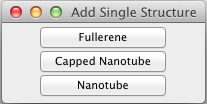
\includegraphics[scale= 0.6]{../../../../screens/nanocap_single_struct_win.png}
%\caption{\nanocap~structure list for adding a single structure}
%\label{n_single_structure_list}
%\end{figure}
%
%An unconstructed nanotube structure will then be added to the structure list:
%
%\begin{figure}[h!]
%\centering
%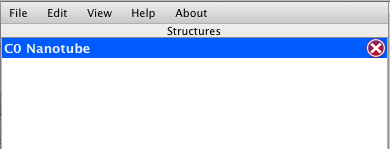
\includegraphics[scale= 0.6]{../../../../screens/nanocap_init_nanotube.png}
%\caption{\nanocap~structure list for adding a single structure}
%\label{init_nanotube}
%\end{figure}
%
%The template nanotube structure has no atoms or dual lattice points. 

To construct the carbon lattice the user has the option for either a finte-length nanotube or one that is periodic along the axial direction. 

 \begin{figure}[h!]
\centering
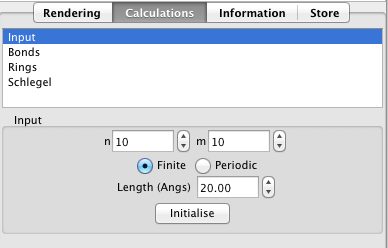
\includegraphics[scale= 0.5]{../../../../screens/nanocap_nanotube_init_finite_win.png}
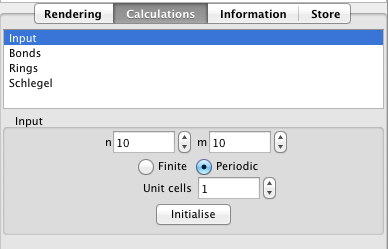
\includegraphics[scale= 0.5]{../../../../screens/nanocap_nanotube_init_periodic_win.png}
\caption{Nanotube construction options}
\label{nanotube_constructure_options}
\end{figure}

\subsubsection{Finite tubes}

Finite tubes are constructed as close to a user defined length as possible. This is done by constructing \textit{strips} of basis points along the chiral vector ($n,m$):

\begin{equation*}
\begin{array}{rl}
 \vect{P}_i  & =  n_i\vect{a_1} + m_i\vect{a_2}\\
 \vect{a_1}  &=  \tfrac{\sqrt{3}a_c}{2} (\sqrt{3}, 1)\\
 \vect{a_2}  &=  \tfrac{\sqrt{3}a_c}{2} (\sqrt{3}, -1)\\
\end{array}
\end{equation*}

\noindent where $a_c$ is the carbon bond length of 1.421~\AA. The incremented values ($n_i,m_i$) range from (0,0) to ($n,m$) and depends on:
\begin{equation*}
\begin{array}{rl}
n_i\verb!++! &\mbox{ if~~$m_i/( 2n_i+m_i)>m/( 2n+m)$} \\
m_i\verb!++! &\mbox{ if~~$m_i/( 2n_i+m_i)\leq m/( 2n+m)$} \\
 \end{array}
\end{equation*}
\noindent After each new row of points, the origin is translated in the $z$ direction by $\sqrt{3}a_c$. The current distance along the nanotube axis is then compared against the user defined length to determine if another strip should be added. The user defined length is inputted in the \textbf{Calculations--$>$Input} options.
 

At each basis point $\vect{P}$ at position $(p_x,p_z)$, the positions of the carbon atoms ($\vect{A}$ and  $\vect{B}$) and dual lattice points ($\vect{D}$) are given by:
\begin{equation*}
\begin{split}
\vect{A} &=  (p_x  , p_z)\\
\vect{B} &=  (p_x +a_c  , p_z)\\
 \vect{D} &=  (p_x + 2a_c , p_z)
 \end{split}
\end{equation*}

 
\subsubsection{Periodic tubes}

Periodic tubes are constructed using a user defined number of unit cells in the \textit{z} direction. The \textbf{periodic length}  $L$ of a nanotube of chirality ($n,m$) with $u$ unit cells is given by:

\begin{equation*}
\begin{split}
L &= u*|\vect{T}|\\
\vect{T}  &= t_1\vect{a_1} + t_2\vect{a_2}
 \end{split}
\end{equation*}
\noindent where the coefficients $t_1$ and $t_2$ have no common divisors except for unity and are given by:
\begin{equation*}
\begin{split}
 t_1 &= (2m + n)/ d_{R} \\
 t_2 &= -(2n + m)/ d_{R} \\
d_{R} &= \texttt{gcd}(2n+m, 2m+n)
 \end{split}
\end{equation*}

During construction the carbon atoms and dual lattice points are constructed as for the finite tubes with the replacement of the user-defined length with the periodic length. After construction, any points surpassing the periodic length are removed.

The number of unit cells can also be found in the \textbf{Calculations--$>$Input} options.

The \textbf{periodic length} can be found in the \textbf{Information} options tab. This will be required by simulation software if the nanotube is to be
used in a periodic simulation.

%\end{document}